\documentclass[hyperref, UTF8]{ctexart}
\usepackage{graphicx}
\usepackage{float}
\usepackage{amsmath}
\usepackage{amsfonts}
\usepackage{amssymb}
\usepackage{fontspec}
\usepackage{tikz}
%\setmonofont{Consolas}
%\setCJKmainfont{Noto Sans S Chinese Regular}
\usetikzlibrary{shapes.geometric, arrows}
\tikzstyle{startstop} = [rectangle, rounded corners, minimum width=3cm, minimum height=1cm,text centered, draw=black, fill=red!30]
\tikzstyle{io} = [trapezium, trapezium left angle=70, trapezium right angle=110, minimum width=3cm, minimum height=1cm, text centered, draw=black, fill=blue!30]
\tikzstyle{process} = [rectangle, minimum width=3cm, minimum height=1cm, text centered, draw=black, fill=orange!30]
\tikzstyle{decision} = [diamond, minimum width=3cm, minimum height=1cm, text centered, draw=black, fill=green!30]
\tikzstyle{arrow} = [thick,->,>=stealth]
\usepackage[a4paper, top=3cm, bottom=3cm, left=3cm, right=3cm]{geometry}
\usepackage{subcaption}
\usepackage{xcolor}
\usepackage{listings}
\lstset{
	keywordstyle=\color{blue!70},
	commentstyle=\color{red!50!green!50!blue!50},
	frame=shadowbox,
	rulesepcolor=\color{red!20!green!20!blue!20},
	tabsize=2,
	basicstyle=\ttfamily\small,
	numberstyle=\tiny,
	numbers=left,
	showstringspaces=false,
	breaklines=true,
	language=MATLAB
}
\hypersetup{
	colorlinks=true,
	bookmarks=true,
	bookmarksopen=true,
	pdftitle=遥感综合实验~图像预处理实验报告,
	pdfauthor=16020710017~蓝彧文,
	linkcolor=blue
}
\title{遥感综合实验实验报告\\遥感图像预处理}
\author{蓝彧文~16020710017}
\begin{document}
	\maketitle
	\tableofcontents
	\newpage
	实验中使用的所有代码和数据可以在\\ \url{https://github.com/EwenLan/remote-sensing-library}获取。
	\section{实验一~图像滤波}
	\subsection{实验目的}
设计和使用低通滤波器,滤除分布在图像中的高斯白噪声。
\subsection{实验原理}
\subsubsection{高斯白噪声}
高斯白噪声是一种理想的噪声模型。高斯白噪声中,噪声振幅值是服从正态分布的。
\[ f(x)=\frac{1}{\sqrt{2\pi}\sigma}\mathrm{e}^{-\frac{(x-\mu)^2}{2\sigma^2}} \]
它的振幅分布直方图如下图\ref{fig:gwnhistogram}所示。
\begin{figure}[H]
	\centering
	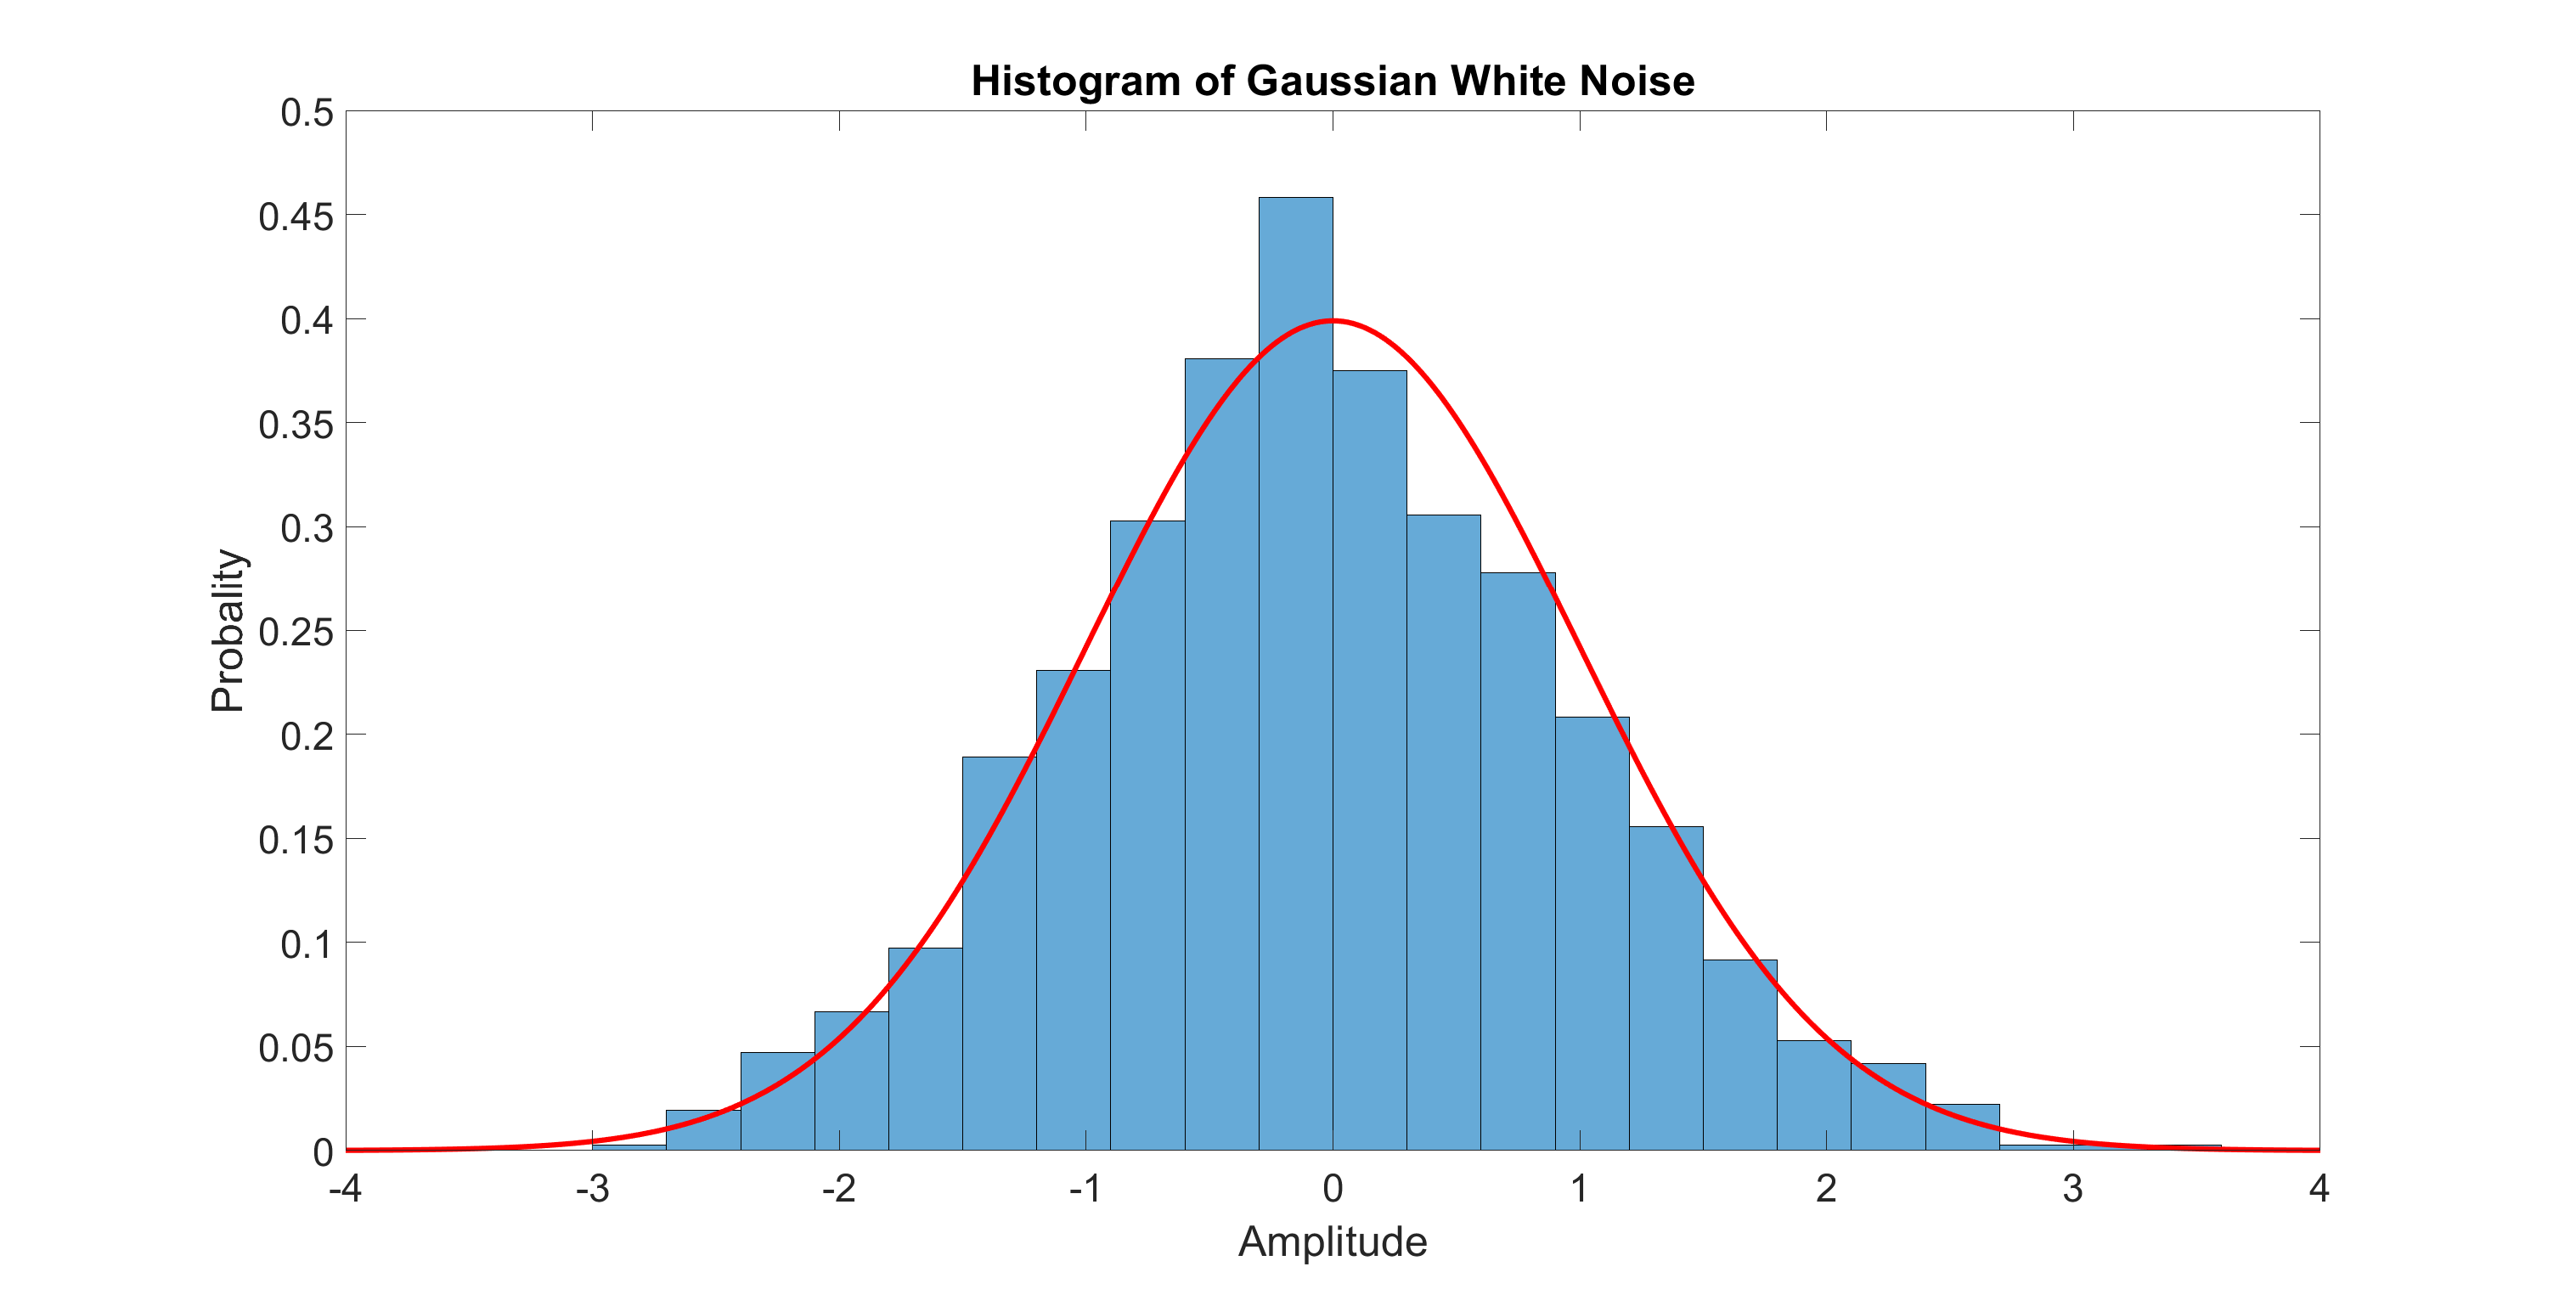
\includegraphics[width=0.7\linewidth]{figure/gwn_histogram}
	\caption{高斯白噪声幅度概率分布}
	\label{fig:gwnhistogram}
\end{figure}
它的功率谱是在频域内均匀分布的,在无限宽频带内满足
\[ G(\omega) = \frac{N_0}{2},\quad -\infty<\omega<+\infty \]
它的自相关函数为为
\[ R(\tau) = \frac{1}{2\pi}\int_{-\infty}^{+\infty}G(\omega)\mathrm{e}^{\mathrm{j}\omega t}\mathrm{d}\omega=\frac{N_0}{2}\delta(\tau) \]

在数字图像中,高斯白噪声线性叠加在图像中。设$f(x, y)$为原图像的表达式,$v(x, y)$为噪声在时空域上的表达式,则包含噪声的图像表达为
\[ g(x, y) = f(x, y) + v(x, y)\]
\subsubsection{傅里叶变换}
傅里叶变换是一种常用的信号分析方法。对于在时空上分布的二数字维图像$f(x, y)$,有傅里叶变换
\[ F(u, v) = \sum_{n = 0}^{N - 1}\sum_{m = 0}^{M - 1}\mathrm{e}^{-\mathrm{j}(\omega_kn+\omega_lm)}f(n, m) \]
\subsubsection{低通滤波器}
\subsection{实验流程}
\subsection{实验程序}
\subsection{实验结果和分析}
	\section{实验二~图像变换}
	\subsection{实验目的}
学习和实践图像翻转、对数变换、幂次变换等图像处理方法。学习使用算术、逻辑操作实现图像增强。
\subsection{实验原理}
\subsubsection{图像反转}
对于二维灰度图像可以执行计算
\[ s=L-1-r \]
重新计算每一个像素点的像素值。这样计算之后得到的图像即为反转后的图像。图像反转会使得原本在图像中是明亮的区域变成黑暗的区域、黑暗的区域变成明亮的区域。
\subsubsection{对数变换}
对于二维灰度图像可以执行计算
\[ s=c\log(1+r) \]
重新计算每一点的像素值。这样的计算,可以提高图像在暗部或明部细节的辨识度。%例如,一个图像的能量主要集中在比较暗的部分,即在图像中暗部保存了许多细节,正常显示的时候会显得图像细节难以辨认。如果对这样的图像进行对数变换,那么就使得暗部的像素点的值得到提升,提高了图像在暗部的可辨识性。
\subsubsection{幂次变换}
对于二维的灰度图像可以执行计算
\[ s=cr^b \]
重新计算每一点的像素值。$c$和$b$为正常数,当$b$取不同值时将得到不同的变换曲线。
\subsubsection{使用算术、逻辑操作进行增强}
对两幅或多幅图像进行计算,进行求比值、求差值计算。可以实现从不同时期的遥感数据中分析出地表特征的变化。
\subsection{实验流程}
本次实验的实验流程如图\ref{fig:rsexp_flowchart}所示
\begin{figure}[H]
	\centering
\begin{tikzpicture}[node distance=1.4cm]
\node(start) [startstop] {开始};
\node(input_img) [io, below of=start] {读取二维灰度图片};
\node(power) [process, below of=input_img] {进行幂次变换};
\node(log) [process, below of=power] {进行对数变换};
\node(plot) [process, below of=log] {绘制变换曲线};
\node(output_img) [io, below of=plot] {输出变换后的图片};
\node(output_graph) [io, below of=output_img] {输出绘制的变换曲线};
\node(input_rsimg) [io, below of=output_graph] {读取具有差异的两幅遥感图像};
\node(process_rsimg) [process, below of=input_rsimg] {选择合适的变换对遥感图像进行处理};
\node(output_rsimg) [io, below of=process_rsimg] {输出处理后的遥感图像};
\node(end) [startstop, below of=output_rsimg] {结束};

\draw[arrow] (start) -- (input_img);
\draw[arrow] (input_img) -- (power);
\draw[arrow] (power) -- (log);
\draw[arrow] (log) -- (plot);
\draw[arrow] (plot) -- (output_img);
\draw[arrow] (output_img) -- (output_graph);
\draw[arrow] (output_graph) -- (input_rsimg);
\draw[arrow] (input_rsimg) -- (process_rsimg);
\draw[arrow] (process_rsimg) -- (output_rsimg);
\draw[arrow] (output_rsimg) -- (end);
\end{tikzpicture}
\caption{图像变换实验流程图}
\label{fig:rsexp_flowchart}
\end{figure}
\subsection{实验程序}
\lstinputlisting[caption={反转变换程序代码}]{"../Executable Script/Exp 2/ReverseTransformAndCompare.m"}
\lstinputlisting[caption={反转变换函数}]{"../Function Library/ReverseTransform.m"}
\lstinputlisting[caption={反转变函数曲线绘制代码}]{"../Executable Script/Exp 2/PlotReverseTransformFunction.m"}
\lstinputlisting[caption={幂次变换程序代码}]{"../Executable Script/Exp 2/GammaTransformAndCompare.m"}
\lstinputlisting[caption={幂次变换函数}]{"../Function Library/GammaTransform.m"}
\lstinputlisting[caption={幂次变换函数曲线绘制函数}]{"../Function Library/PlotGammaTransformFunction.m"}
\lstinputlisting[caption={对数变换程序代码}]{"../Executable Script/Exp 2/LogTransformAndCompare.m"}
\lstinputlisting[caption={对数变换函数}]{"../Function Library/LogTransform.m"}
\lstinputlisting[caption={对数变换函数曲线绘制函数}]{"../Function Library/PlotLogTransformFunction.m"}
\lstinputlisting[caption={遥感图像变化检测}]{"../Executable Script/Exp 2/CompareTwoImages.m"}
\lstinputlisting[caption={自动二值化图像函数}]{"../Function Library/AutoBinarizeImage.m"}
\subsection{实验结果和分析}
\begin{figure}[H]
	\centering
	\begin{minipage}{0.45\linewidth}
		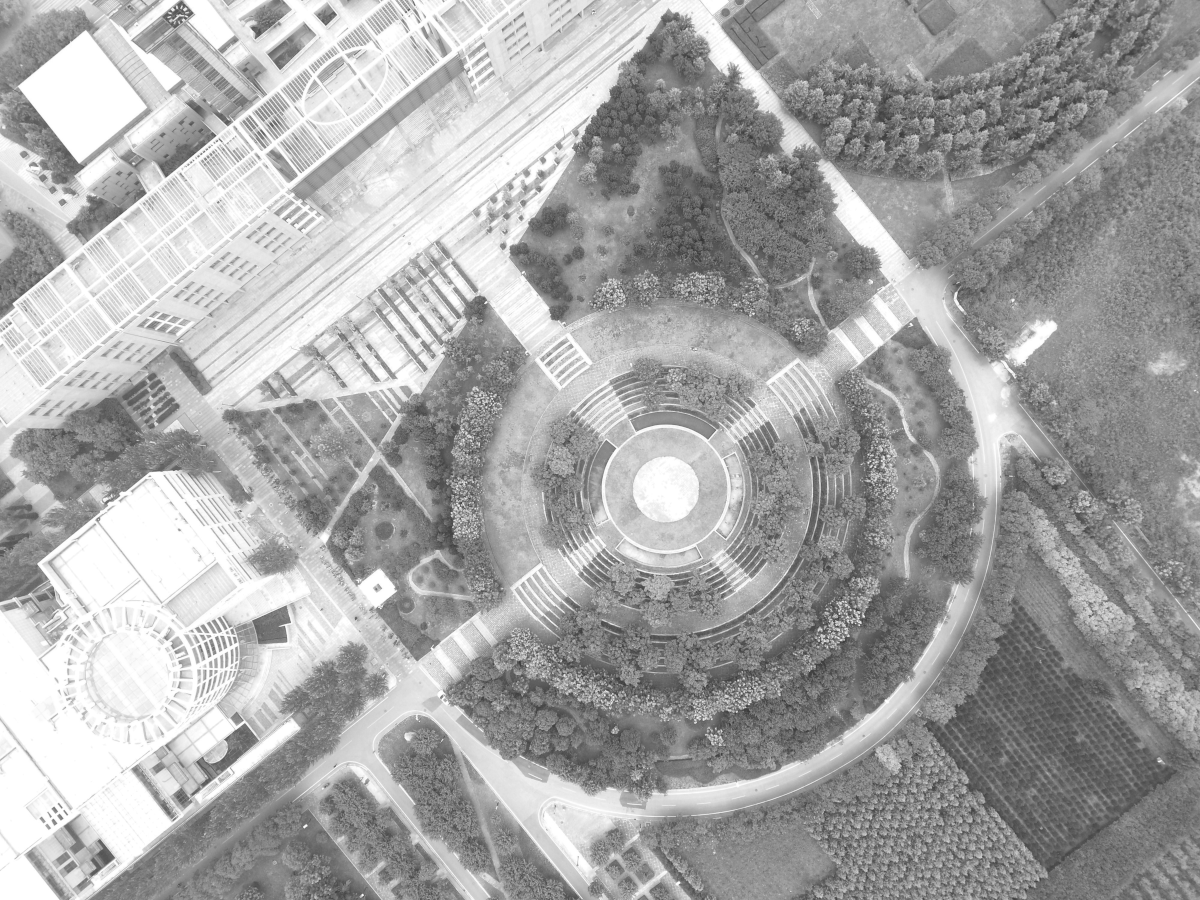
\includegraphics[width=\linewidth]{figure/DJI_0027_Gray.png}
		\caption{原图片}
		\label{fig:transform_original}
	\end{minipage}
	\begin{minipage}{0.45\linewidth}
		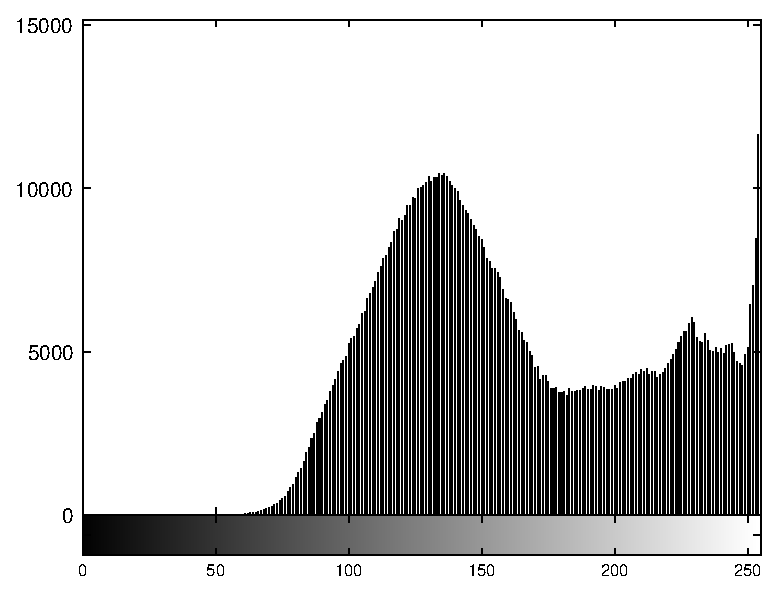
\includegraphics[width=\linewidth]{figure/DJI_0027_Histogram}
		\caption{原图片统计直方图}
		\label{fig:dji0027histogram}
	\end{minipage}
\end{figure}
\subsubsection{反转变换}
\begin{figure}[H]
	\centering
	\begin{minipage}{0.45\linewidth}
		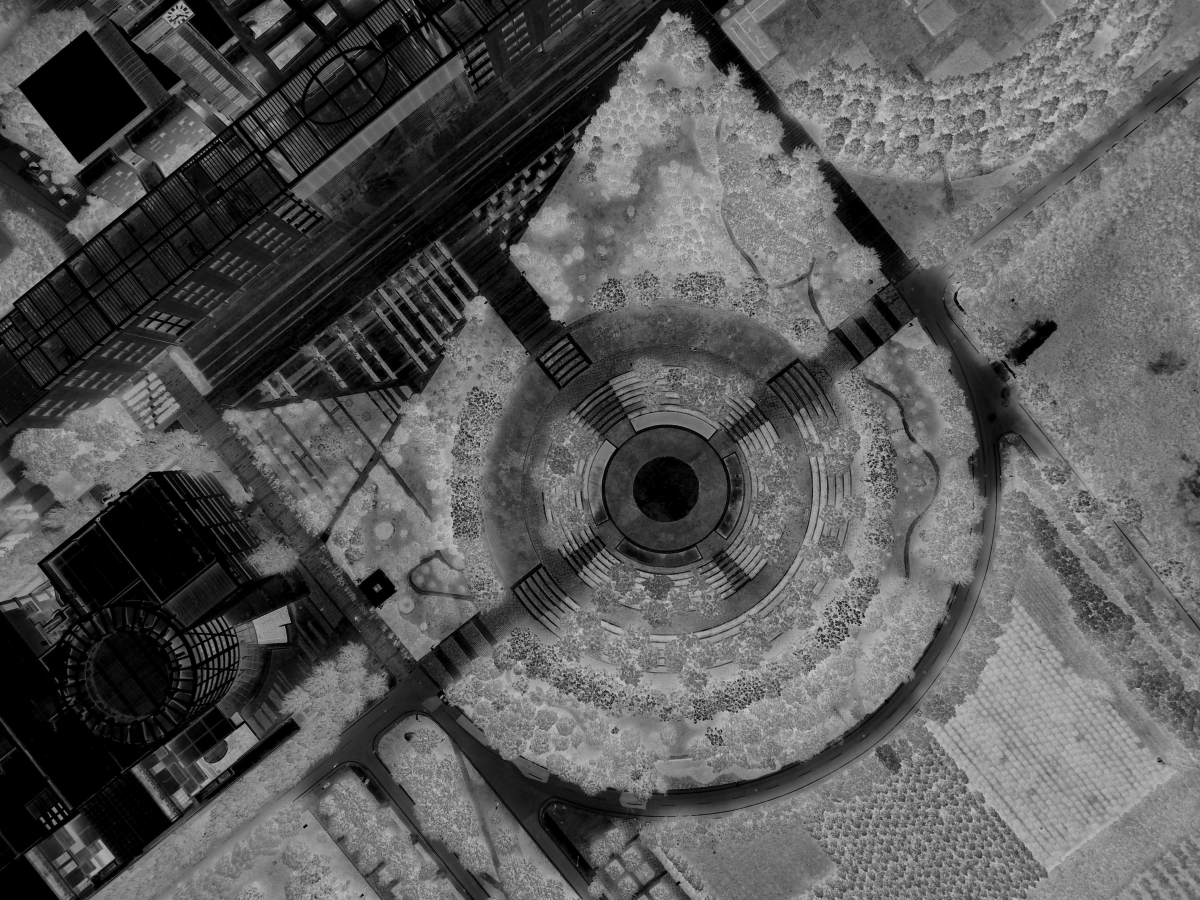
\includegraphics[width=\linewidth]{figure/DJI_0027_Reversed.png}
		\caption{$s=L-1-r$的反转变换}
	\end{minipage}
	\begin{minipage}{0.45\linewidth}
		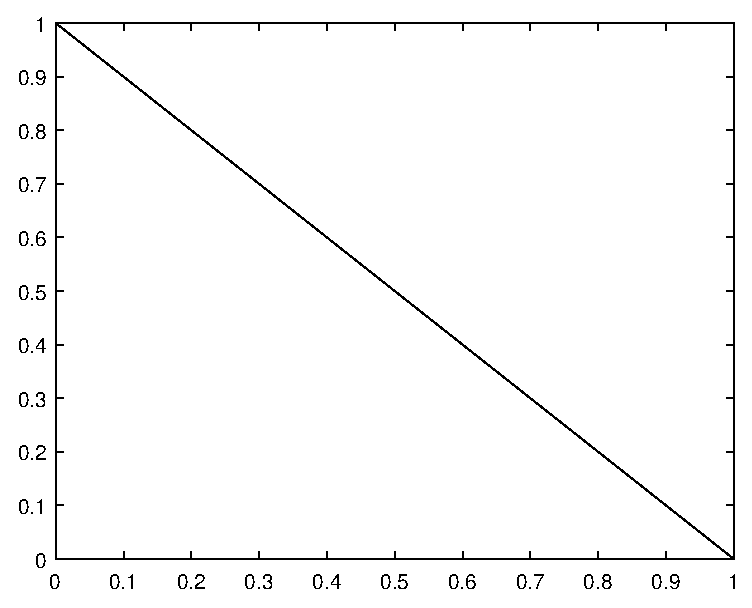
\includegraphics[width=\linewidth]{figure/DJI_0027_Reversed_Graph.eps}
		\caption{$s=L-1-r$变换曲线}
	\end{minipage}
\end{figure}
\subsubsection{幂次变换}
$b=1$的幂次变换
\begin{figure}[H]
	\centering
	\begin{minipage}{0.45\linewidth}
		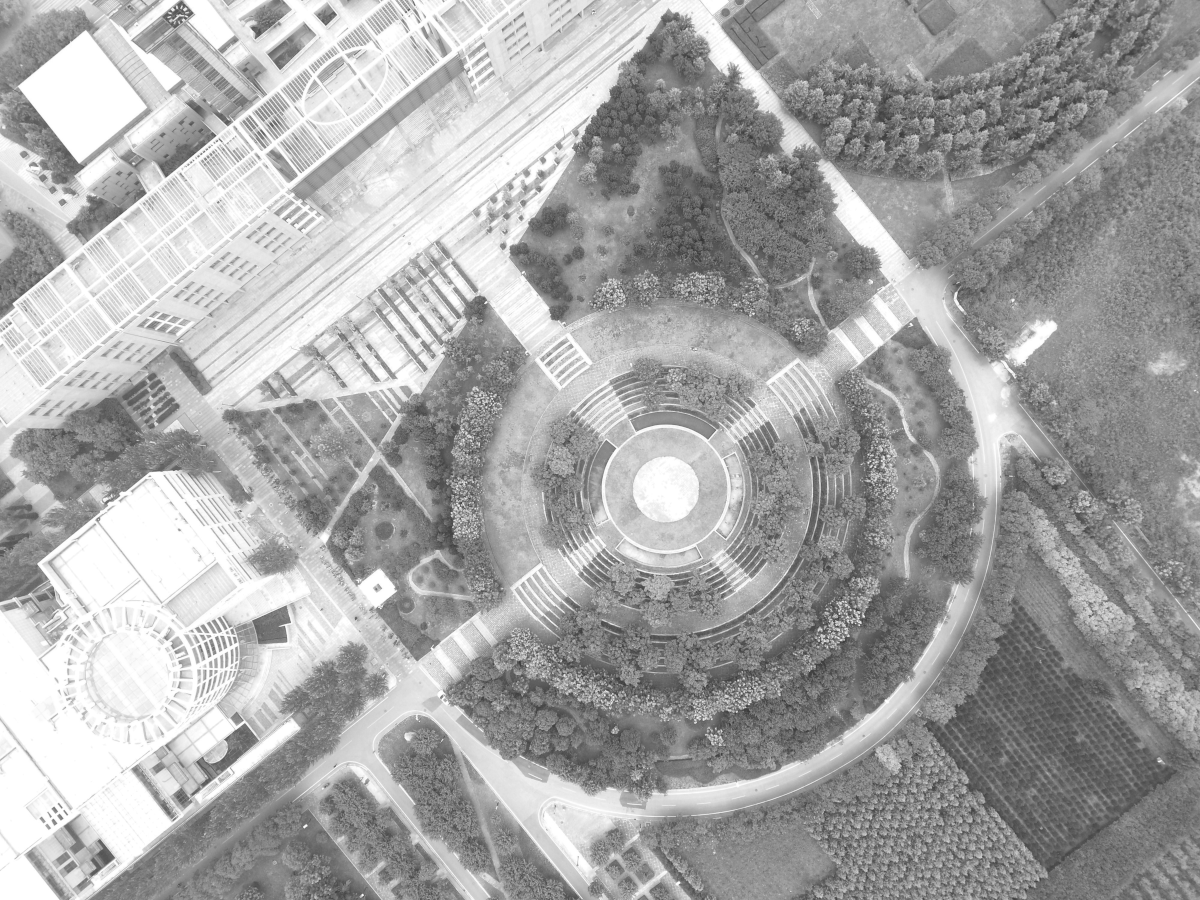
\includegraphics[width=\linewidth]{figure/DJI_0027_Gamma_100.png}
		\caption{$s=1r^1$的幂次变换}
	\end{minipage}
	\begin{minipage}{0.45\linewidth}
		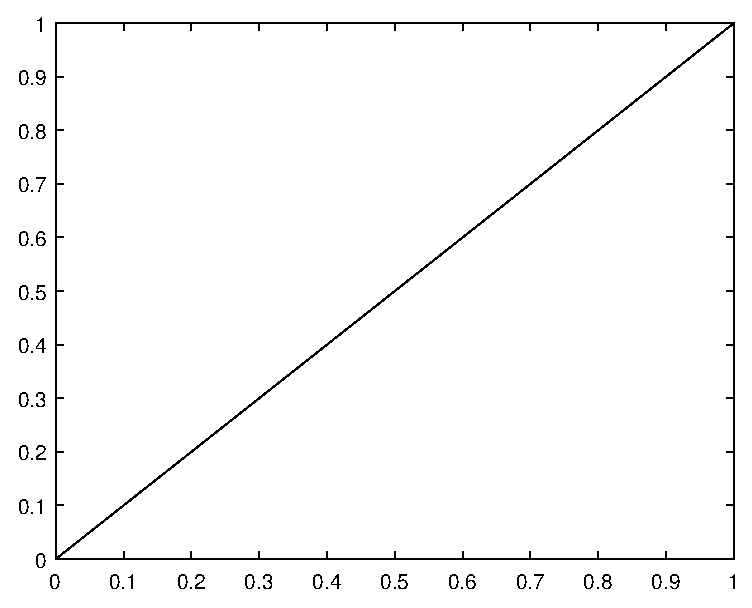
\includegraphics[width=\linewidth]{figure/DJI_0027_Gamma_100_Graph.eps}
		\caption{$s=1r^1$变换曲线}
	\end{minipage}
\end{figure}

$b=0.5$的幂次变换
\begin{figure}[H]
	\centering
	\begin{minipage}{0.45\linewidth}
		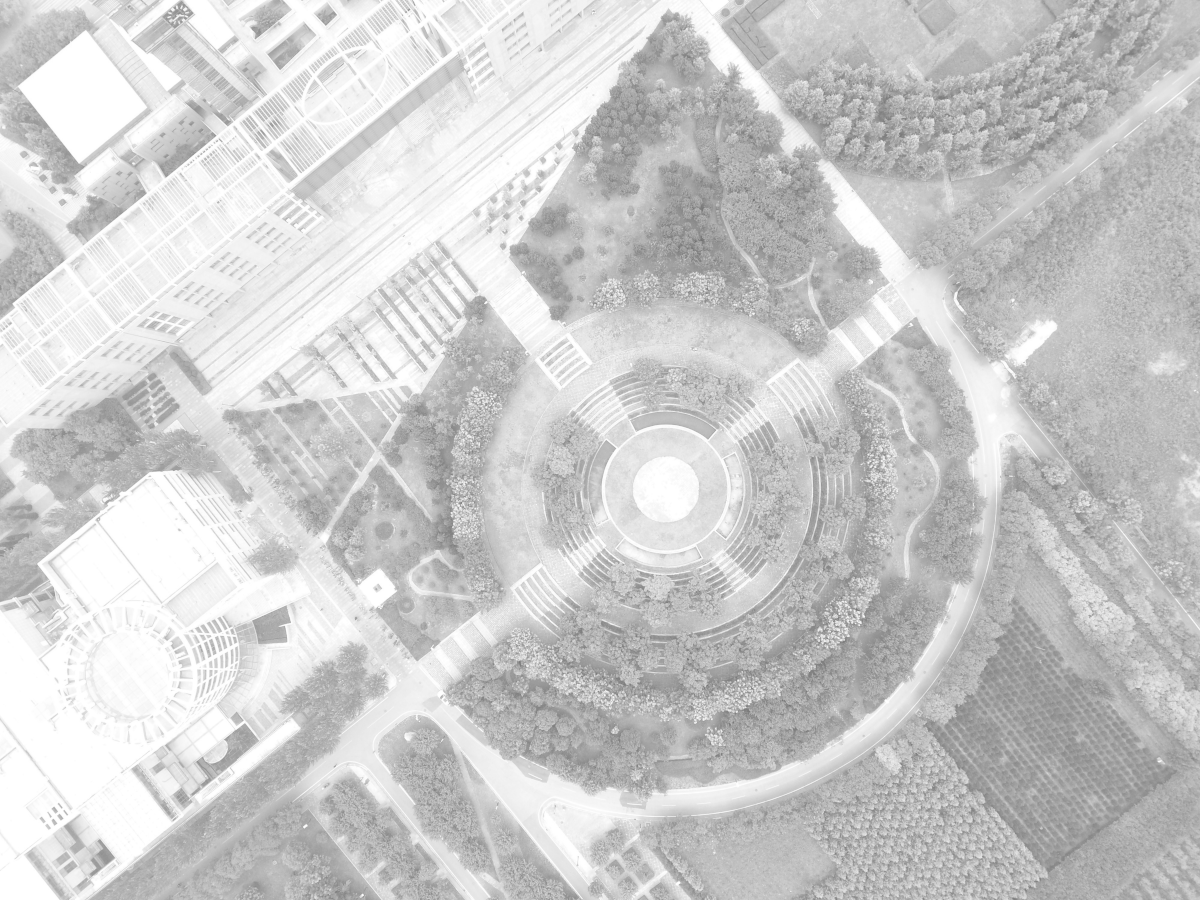
\includegraphics[width=\linewidth]{figure/DJI_0027_Gamma_50.png}
		\caption{$s=1r^0.5$的幂次变换}
	\end{minipage}
	\begin{minipage}{0.45\linewidth}
		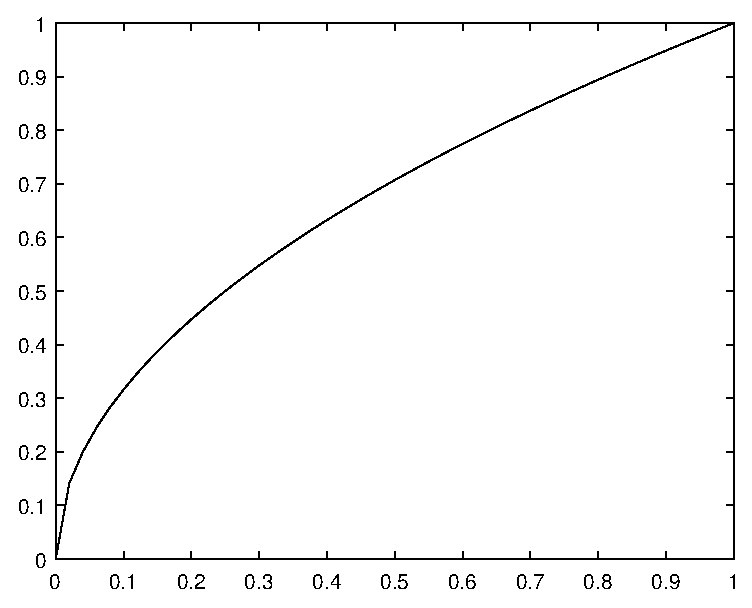
\includegraphics[width=\linewidth]{figure/DJI_0027_Gamma_50_Graph.eps}
		\caption{$s=1r^{0.5}$变换曲线}
	\end{minipage}
\end{figure}

$b=2$的幂次变换
\begin{figure}[H]
	\centering
	\begin{minipage}{0.45\linewidth}
		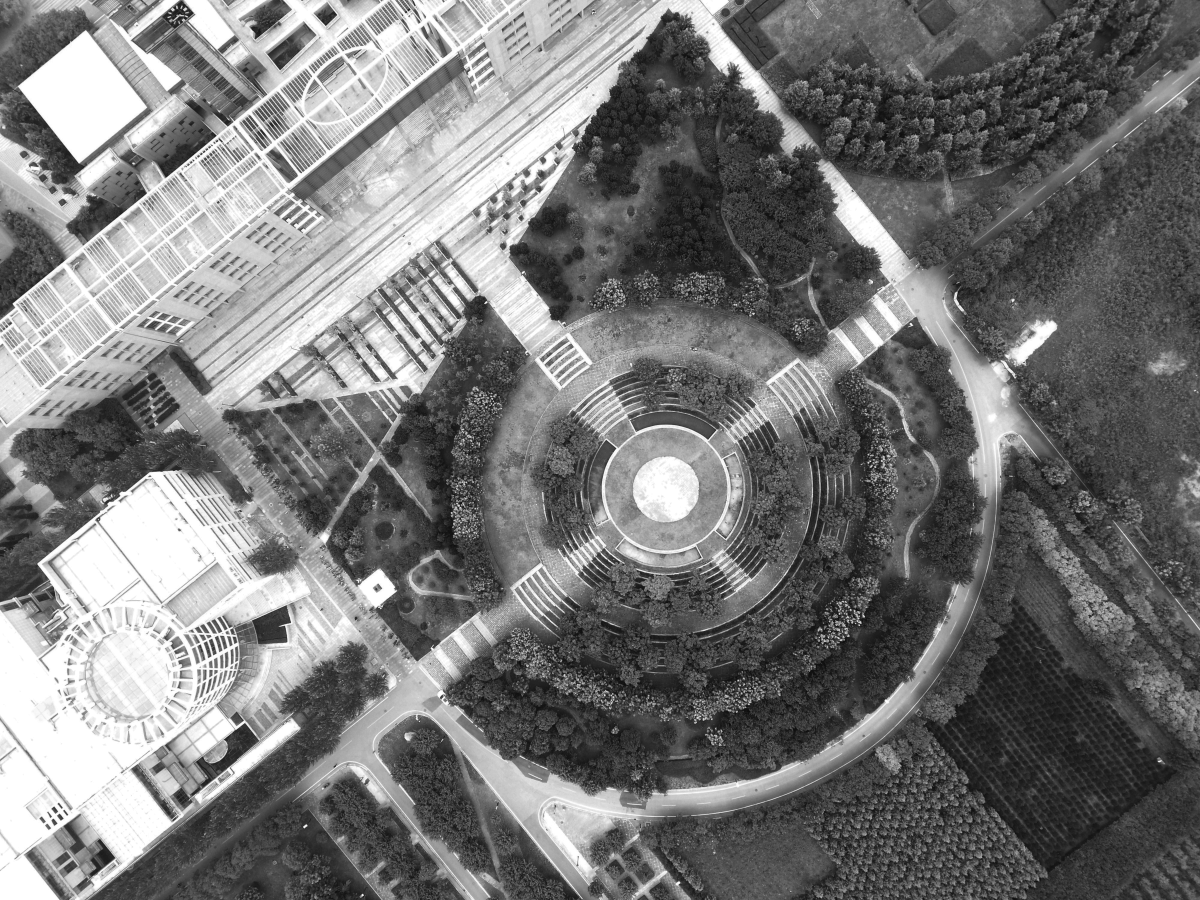
\includegraphics[width=\linewidth]{figure/DJI_0027_Gamma_200.png}
		\caption{$s=1r^2$的幂次变换}
	\end{minipage}
	\begin{minipage}{0.45\linewidth}
		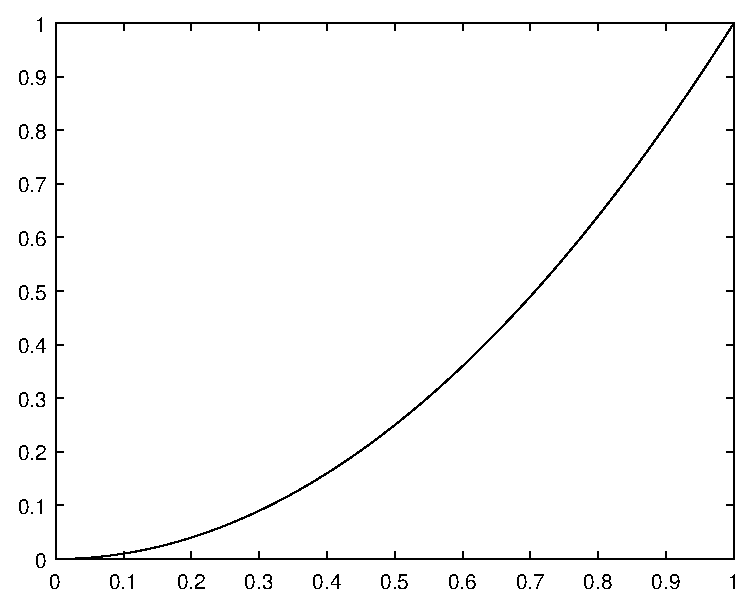
\includegraphics[width=\linewidth]{figure/DJI_0027_Gamma_200_Graph.eps}
		\caption{$s=1r^2$变换曲线}
	\end{minipage}
\end{figure}
\subsubsection{对数变换}
$c=1$的对数变换
\begin{figure}[H]
	\centering
	\begin{minipage}{0.45\linewidth}
		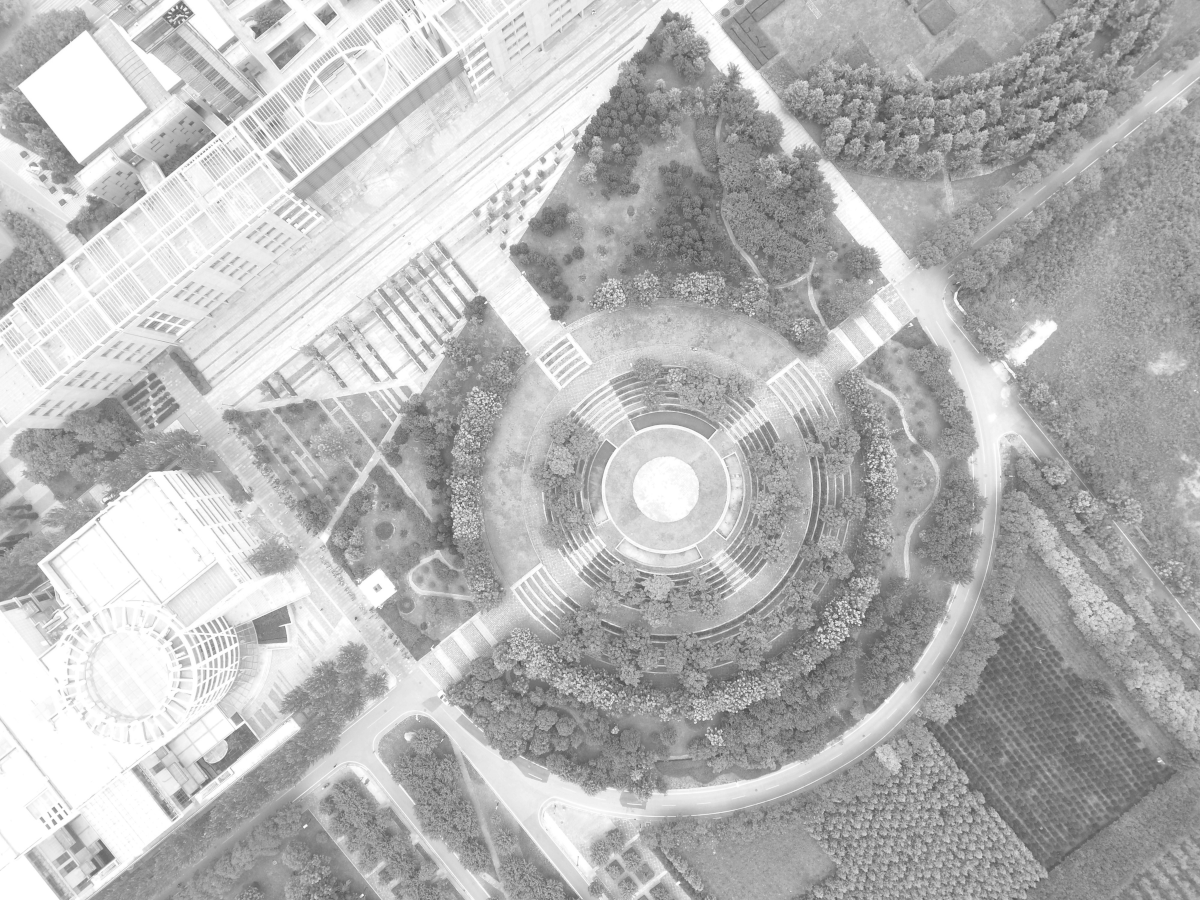
\includegraphics[width=\linewidth]{figure/DJI_0027_Log_100.png}
		\caption{$s=\log_2(1+1r)$的对数变换}
	\end{minipage}
	\begin{minipage}{0.45\linewidth}
		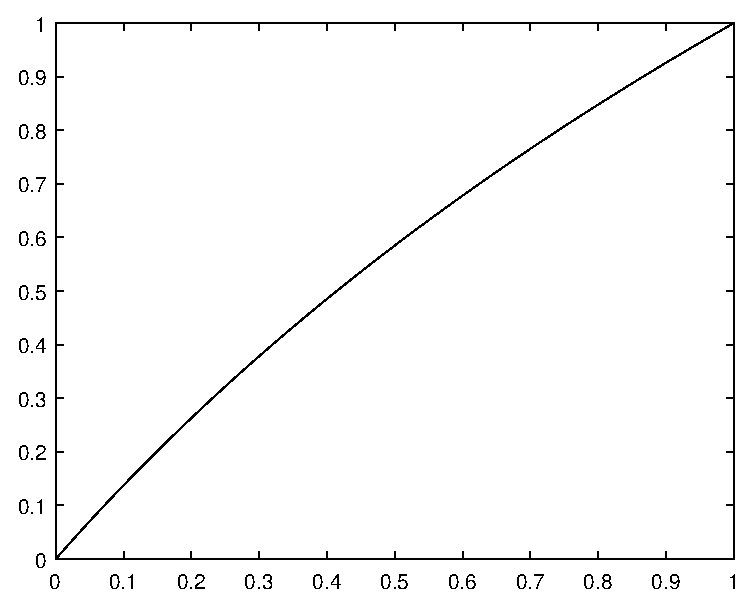
\includegraphics[width=\linewidth]{figure/DJI_0027_Log_100_Graph.eps}
		\caption{$s=\log_2(1+1r)$变换曲线}
	\end{minipage}
\end{figure}

$c=10$的对数变换
\begin{figure}[H]
	\centering
	\begin{minipage}{0.45\linewidth}
		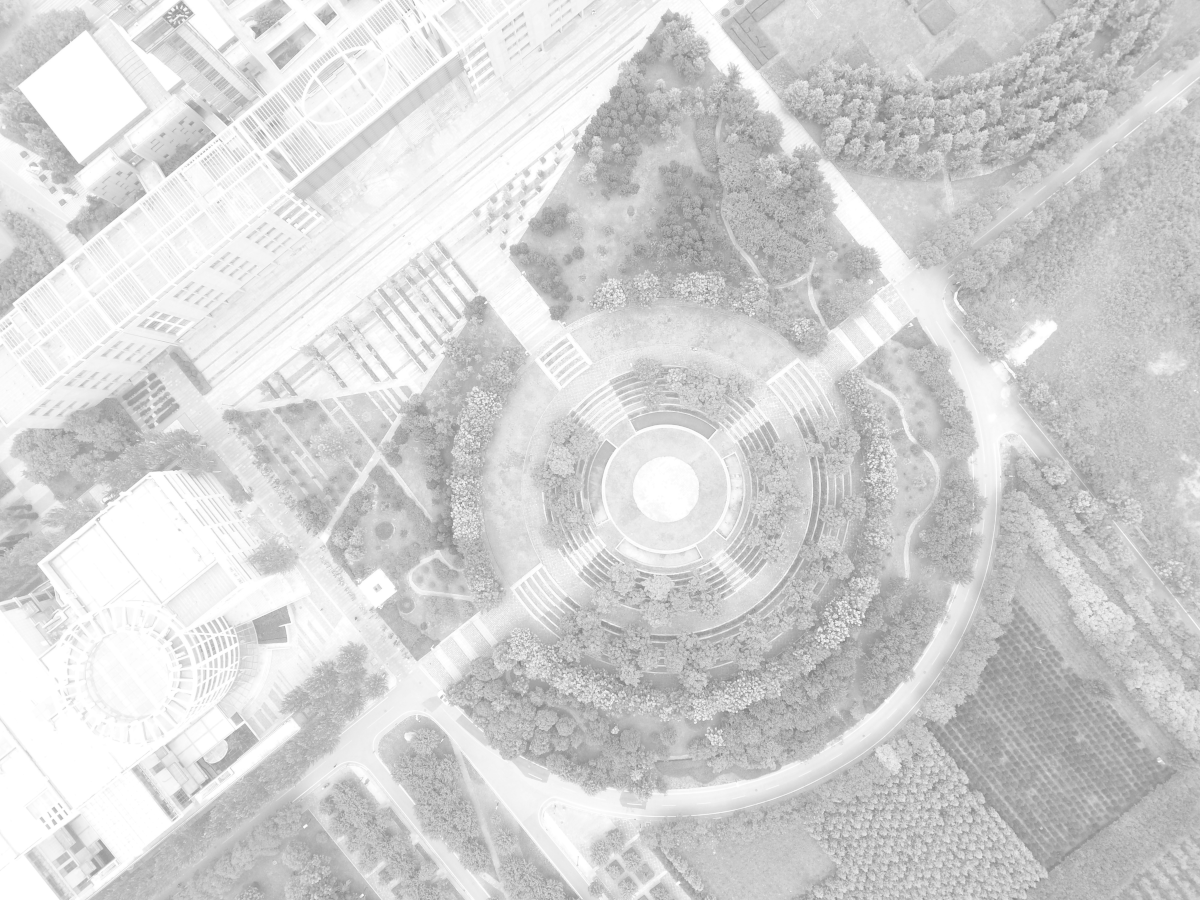
\includegraphics[width=\linewidth]{figure/DJI_0027_Log_1000.png}
		\caption{$s=\log_{11}(1+10r)$的对数变换}
	\end{minipage}
	\begin{minipage}{0.45\linewidth}
		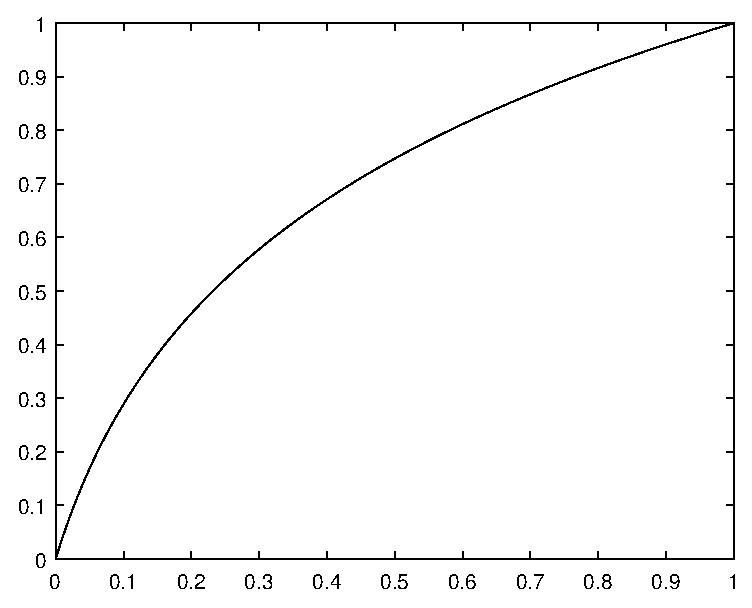
\includegraphics[width=\linewidth]{figure/DJI_0027_Log_1000_Graph.eps}
		\caption{$s=\log_{11}(1+10r)$变换曲线}
	\end{minipage}
\end{figure}

$c=-0.9$的对数变换
\begin{figure}[H]
	\centering
	\begin{minipage}{0.45\linewidth}
		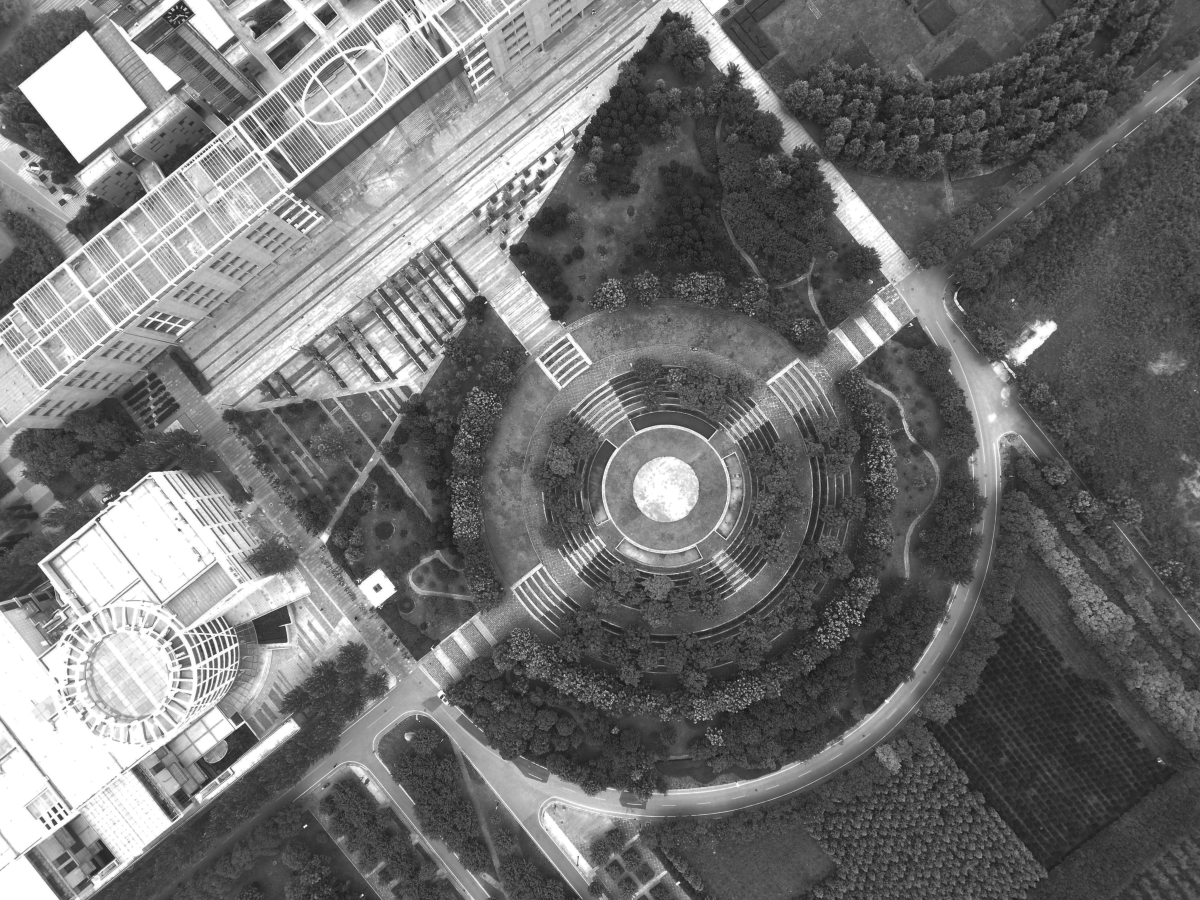
\includegraphics[width=\linewidth]{figure/DJI_0027_Log_-90.png}
		\caption{$s=\log_{0.1}(1-0.9r)$的对数变换}
	\end{minipage}
	\begin{minipage}{0.45\linewidth}
		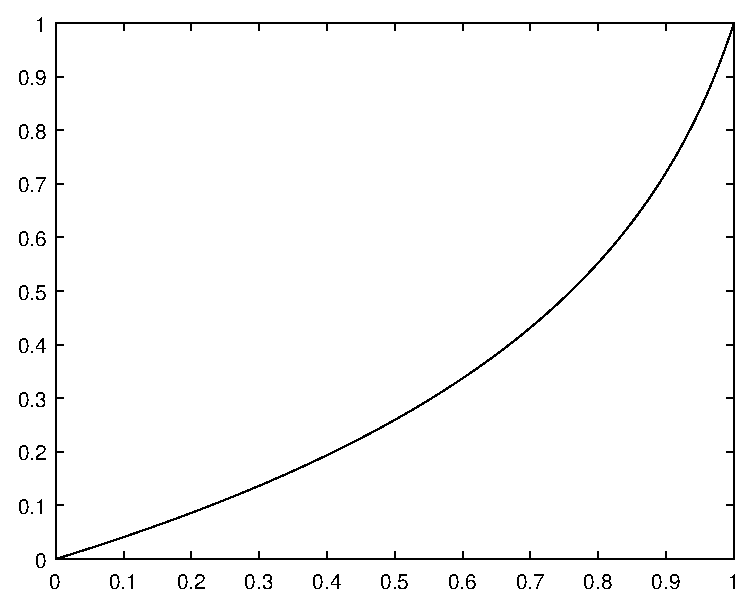
\includegraphics[width=\linewidth]{figure/DJI_0027_Log_-90_Graph.eps}
		\caption{$s=\log_{0.1}(1-0.9r)$变换曲线}
	\end{minipage}
\end{figure}
\subsubsection{遥感图像变化检测}
\begin{figure}[H]
	\centering
	\begin{minipage}{0.45\linewidth}
		\includegraphics[width=\linewidth]{figure/san_gt.bmp}
		\caption{示例变化检测}
	\end{minipage}
	\begin{minipage}{0.45\linewidth}
		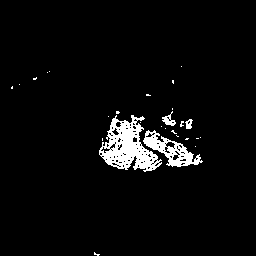
\includegraphics[width=\linewidth]{figure/exp2compare.png}
		\caption{自主实现的变化检测}
	\end{minipage}
\end{figure}
	\section{实验三~图像融合}
	\subsection{实验目的}
掌握一些基本的图像融合方法,包括基于像素灰度值的简单图像融合算法,以及彩色图像的分解于合成。完成遥感图像的图像融合。
\subsection{实验原理}
\subsubsection{图像融合的概念}
综合和提取两个或多个圆的图像信息,获得对同一场景或者目标更为准确、全面、可靠的图像,使之更适合人眼感知或计算机后续处理。
\begin{figure}[H]
	\centering
	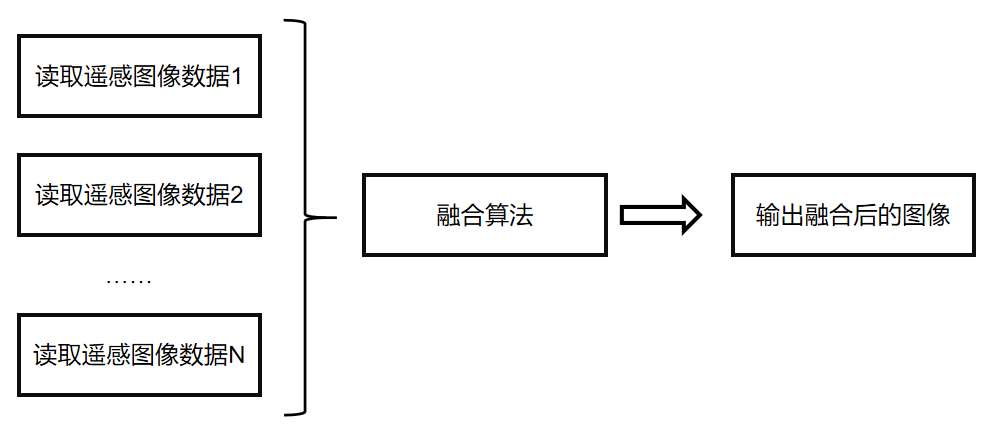
\includegraphics[width=0.7\linewidth]{figure/fusion_flowchart.png}
	\caption{图像融合算法流程图}
	\label{fig:fusion_flowchart}
\end{figure}
\subsubsection{简单的图像融合算法}
\begin{description}
	\item[像素灰度值平均或加权平均法]
	\[ I(x, y)=\frac{\sum_{n=1}^{N}W^n(x, y)I^n(x, y)}{\sum_{n=1}^{N}W^n(x, y)} \]
	\[ W^n(x, y)=\frac{1}{N} \]
	\item[像素灰度值选大法] 
	\[ I(x, y)=\max_n\{I^n(x, y),\quad n=1,2,\dots N\} \]
	\item[像素灰度值选小法] 
	\[ I(x, y)=\min_n\{I^n(x, y),\quad 1,2,\dots N\} \]
\end{description}
\subsubsection{彩色图像的分解与合成}
\begin{description}
	\item[能量图像] 
	\[ I=Ir+Ig+Ib \]
	\item[变换后的彩色图像合成]
	蓝色分量:加高斯噪声污染
	
	绿色分量:进行对数变换
	
	红色分量:进行图像反转
	
	重新合成彩色图像
\end{description}
\subsubsection{彩色图像合成}
通过图像变换与融合突出图像中感兴趣的目标。
\subsubsection{通过图像融合得到变化检测差异图}
\begin{description}
	\item[差异图像] 
	\[ I1=1-\min \left( \frac{\mu_1}{\mu_2},\frac{\mu_2}{\mu_1} \right)  \]
	\[ I2= \left| \log\frac{X_2}{X_1} \right| = \left| \log X_2 - \log X_1 \right|  \]
	\item[图像融合]
	两个差异图的低频成分平均融合,高频成分取小融合。
\end{description}
\subsection{实验流程}
\begin{figure}[H]
	\centering
	\begin{tikzpicture}[node distance=1.5cm]
	\node(start) [startstop] {开始};
	\node(inputimg) [io, below of=start] {读取图片};
	\node(separateimg) [process, below of=inputimg] {分离彩色图像颜色通道};
	\node(fusionchannels) [process, below of=separateimg] {加权合并各通道能量};
	\node(outputenergyimg) [io, below of=fusionchannels] {输出能量合成图像};
	\node(channelcompare) [process, below of=outputenergyimg] {使用图片的两个不同通道进行对比};
	\node(outputchannelcomparation) [io, below of=channelcompare] {输出比较的结果};
	\node(channeltransform) [process, below of=outputchannelcomparation] {对各个通道分别进行变换};
	\node(outputtransformed) [io, below of=channeltransform] {输出变换后的图像};
	\node(inputmask) [io, below of=outputtransformed] {输入兴趣区域蒙版};
	\node(interestedarea) [process, below of=inputmask] {合成兴趣区域图像};
	\node(outputinterestedarea) [io, below of=interestedarea] {输出兴趣区域图像};
	\node(end) [startstop, below of=outputinterestedarea] {结束};
	
	\draw[arrow] (start) -- (inputimg);
	\draw[arrow] (inputimg) -- (separateimg);
	\draw[arrow] (separateimg) -- (fusionchannels);
	\draw[arrow] (fusionchannels) -- (outputenergyimg);
	\draw[arrow] (outputenergyimg) -- (channelcompare);
	\draw[arrow] (channelcompare) -- (outputchannelcomparation);
	\draw[arrow] (outputchannelcomparation) -- (channeltransform);
	\draw[arrow] (channeltransform) -- (outputtransformed);
	\draw[arrow] (outputtransformed) -- (inputmask);
	\draw[arrow] (inputmask) -- (interestedarea);
	\draw[arrow] (interestedarea) -- (outputinterestedarea);
	\draw[arrow] (outputinterestedarea) -- (end);
	\end{tikzpicture}
\end{figure}
\subsection{实验程序}
\lstinputlisting[caption={简单像素加权融合程序}]{"../Executable Script/Exp 3/ColorImageEnergyGraph.m"}

\subsection{实验结果和分析}
\begin{figure}[H]
	\centering	
	\begin{minipage}{0.45\linewidth}
		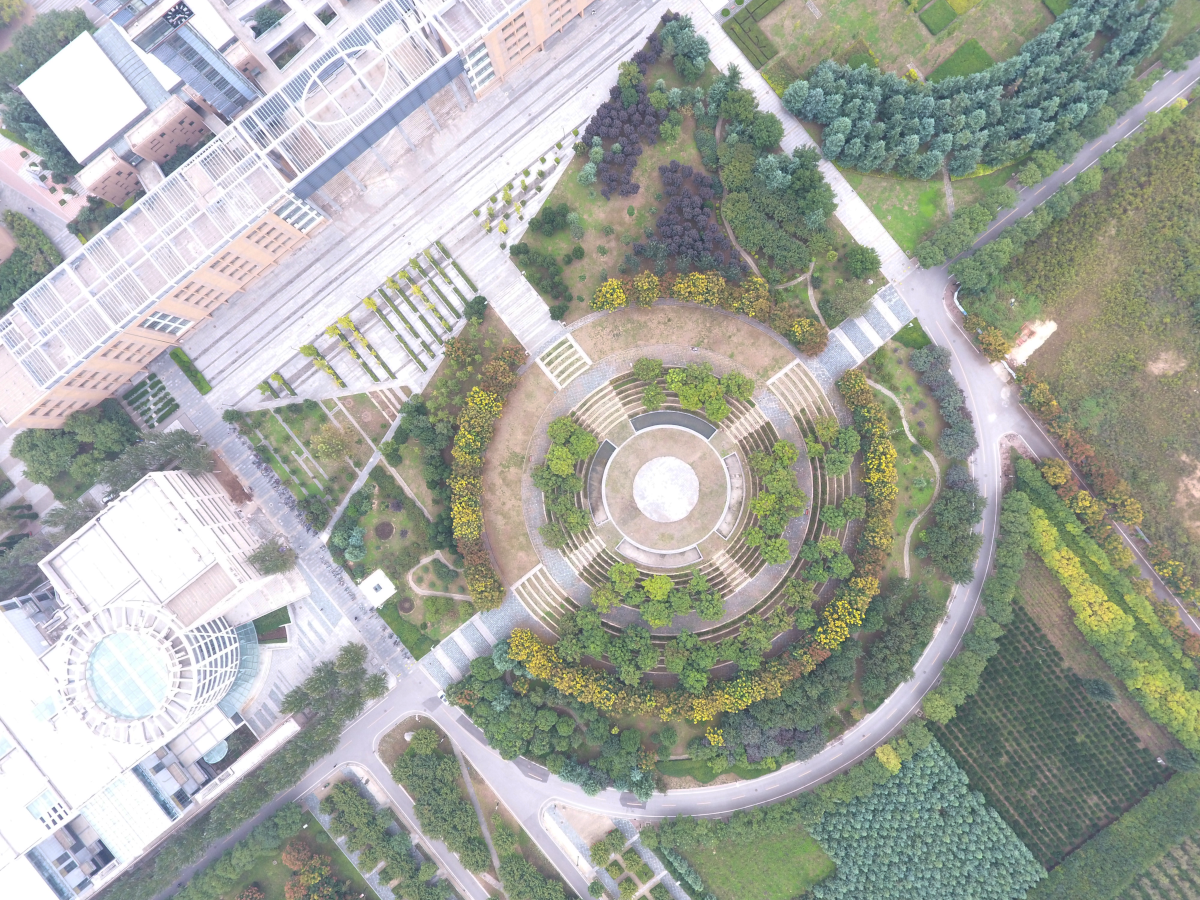
\includegraphics[width=\linewidth]{figure/DJI_0027_Compressed.png}
		\caption{原图片}
	\end{minipage}
	\begin{minipage}{0.45\linewidth}
		\includegraphics[width=\linewidth]{figure/DJI_0027_Energy.png}
		\caption{简单像素加权融合结果}
	\end{minipage}

\end{figure}
\end{document}